%%%%%%%%%%%%%%%%%%%%%%%%%%%%%%%%%%%%%%%%%%%%%%%%%%%%%%%%%%%%%%%%%%%%%%%%%%%%%%%%
%%%%%%%%%%%%%%%%%%   Vorlage für ein Praktikumsprotokoll   %%%%%%%%%%%%%%%%%%%%%
%%%%%%%%%%%%%%%%%%%%%%%%%%%%%%%%%%%%%%%%%%%%%%%%%%%%%%%%%%%%%%%%%%%%%%%%%%%%%%%%

% Erstellt von Maximilian Nöthe, <maximilian.noethe@tu-dortmund.de>
% angepasst von Paul Becker, <paul.becker@tu-dortmund.de>
% ausgelegt für lualatex und Biblatex mit biber

% Kompilieren mit 
% lualatex dateiname.tex
% biber dateiname.bcf
% lualatex dateiname.tex
% lualatex dateiname.tex
% oder einfach mit:
% make

\documentclass[
  tucolor,
  BCOR=12mm,     % 12mm binding corrections, adjust to fit your binding
  parskip=half,  % new paragraphs start with half line vertical space
  open=any,      % chapters start on both odd and even pages
  cleardoublepage=plain,  % no header/footer on blank pages
]{../template/tudothesis}


% Warning, if another latex run is needed
\usepackage[aux]{rerunfilecheck}

% just list chapters and sections in the toc, not subsections or smaller
\setcounter{tocdepth}{1}

%------------------------------------------------------------------------------
%------------------------------ Sprache und Schrift: --------------------------
%------------------------------------------------------------------------------
\usepackage{fontspec}
\defaultfontfeatures{Ligatures=TeX}  % -- becomes en-dash etc.

% german language
\usepackage{polyglossia}
\setdefaultlanguage{german}

% for english abstract and english titles in the toc
\setotherlanguages{english}

% intelligent quotation marks, language and nesting sensitive
\usepackage[autostyle]{csquotes}

% microtypographical features, makes the text look nicer on the small scale
\usepackage{microtype}

%------------------------------------------------------------------------------
%------------------------ Für die Matheumgebung--------------------------------
%------------------------------------------------------------------------------

\usepackage{amsmath}
\usepackage{amssymb}
\usepackage{mathtools}

% Enable Unicode-Math and follow the ISO-Standards for typesetting math
\usepackage[
  math-style=ISO,
  bold-style=ISO,
  sans-style=italic,
  nabla=upright,
  partial=upright,
]{unicode-math}
\setmathfont{Latin Modern Math}

% nice, small fracs for the text with \sfrac{}{}
\usepackage{xfrac}  


%------------------------------------------------------------------------------
%---------------------------- Numbers and Units -------------------------------
%------------------------------------------------------------------------------

\usepackage[
  locale=DE,
  separate-uncertainty=true,
  per-mode=symbol-or-fraction,
]{siunitx}
\sisetup{math-micro=\text{µ},text-micro=µ}

%------------------------------------------------------------------------------
%-------------------------------- tables  -------------------------------------
%------------------------------------------------------------------------------

\usepackage{booktabs}       % stellt \toprule, \midrule, \bottomrule

%------------------------------------------------------------------------------
%-------------------------------- graphics -------------------------------------
%------------------------------------------------------------------------------

\usepackage{graphicx}
\usepackage{grffile}

% allow figures to be placed in the running text by default:
\usepackage{scrhack}
\usepackage{float}
\floatplacement{figure}{htbp}
\floatplacement{table}{htbp}

% keep figures and tables in the section
\usepackage[section, below]{placeins}


%------------------------------------------------------------------------------
%---------------------- customize list environments ---------------------------
%------------------------------------------------------------------------------

\usepackage{enumitem}

%------------------------------------------------------------------------------
%------------------------------ Bibliographie ---------------------------------
%------------------------------------------------------------------------------

\usepackage[
  backend=biber,   % use modern biber backend
  autolang=hyphen, % load hyphenation rules for if language of bibentry is not
                   % german, has to be loaded with \setotherlanguages
                   % in the references.bib use langid={en} for english sources
]{biblatex}
\addbibresource{references.bib}  % die Bibliographie einbinden
\DefineBibliographyStrings{german}{andothers = {{et\,al\adddot}}} 

%------------------------------------------------------------------------------
%------------------------------ Sonstiges: ------------------------------------
%------------------------------------------------------------------------------

\usepackage[pdfusetitle,unicode,linkbordercolor=tugreen]{hyperref}
\usepackage{bookmark}
\usepackage[shortcuts]{extdash}

%------------------------------------------------------------------------------
%-------------------------    Angaben zur Arbeit   ----------------------------
%------------------------------------------------------------------------------

\author{Paul Becker u. Alina Esfani}
\title{optisches Pumpen}
\date{2014}
\chair{Physikalisches Praktikum}
\submissiondate{31. September 2015}

\begin{document}
\frontmatter
\maketitle


\mainmatter
% Hier beginnt der Inhalt mit Seite 1 in arabischen Ziffern
\section{Zielsetzung}
Durch Messung des Transmissionskoeffizienten von Rubidiumgas bei Anlegen eines externen Magnetfeldes wird die
Stärke des Erdmagnetfeldes, die Lande-Faktoren und die Spins der Elektronenhülle und des Kerns der Rubidiumisotope
Rb-85 und Rb-87 berechnet.

\section{Theorie}

Für die beiden verwendeten Rubidiumisotope sind Hyperfeinstruktur- und Zeeman-Aufspaltung unterschiedlich. Die damit
verbundenen Kenngrößen - der Landefaktor, das gyromagnetische Verhältnis und der Spin - können mit Hilfe optischen
Pumpens aufgrund der unterschiedlichen Enerdifferenzen sehr präzise gemessen werden.

\subsubsection{Aufspaltung von Energieniveaus}

Quantenzahlen beschreiben Zustand eines Systems. Durch Kernspin und externes Magentfeld kommt es zu Hyperfeinstruktur-
und Zeemann-Aufspaltung.
Der Gesamtdrehimpuls der Elektronenhülle $\vec{J}$ ist über
\begin{equation}
  \vec{\mu}_\text{J} = -g_\text{J}\mu_\text{B}\vec{J} \quad \text{bzw.} \quad |\vec{\mu}_\text{J}| = -g_\text{J}\mu_\text{B}\sqrt{J (J + 1)}
  \label{magnMom}
\end{equation}
mit einem magnetischen Moment verknüpft, dabei ist $\mu_\text{B}$ das Bohrsche Magneton. Das magnetische Moment der gesamten
Elektronenhülle setzt sich aus den magnetischen Momenten von Bahndrehimpuls $\vec{L}$ und Spin $\vec{S}$ zusammen:
\begin{equation}
  \vec{\mu}_\text{J} = \vec{\mu}_\text{L} + \vec{\mu}_\text{S} \quad \text{mit} \quad |\vec{\mu}_\text{J}| = \mu_\text{B}\sqrt{L (L + 1)} \quad \text{und}
  \quad |\vec{\mu}_\text{S}| = g_\text{S}\mu_\text{B}\sqrt{S (S + 1)}.
\end{equation}
$g_\text{S}$ ist der Lande-Faktor des freien Elektrons, der Zusammenhang der magnetischen Momente wird durch den Lande-Faktor
$g_\text{J}$ ausgedrückt.
%$\vec{\mu}_J$ präzediert um $\vec{J}$, sodass für den Betrag gilt:
%\begin{align}
%  \begin{split}
%    |\vec{\mu}_J| &= |\vec{\mu}_L|\cos\beta + |\vec{\mu}_S|\cos\alpha\\
%    \equiv g_J\mu_B\sqrt{J (J + 1)} = & \mu_B\sqrt{L (L + 1)}\cos\beta + g_S\mu_B\sqrt{S (S + 1)}\cos\alpha
%  \end{split}
%\end{align}
Dieser kann aus den Quantenzahlen über
\begin{equation}
  g_\text{J} = \frac{3.0023J(J+1) + 1.0023[S(S+1) - L(L+1)]}{2J(J+1)}
\end{equation}
berechnet werden.

Liegt ein äußeres Magnetfeld an, kommt es zu einer Aufspaltung der Energieniveaus, da das magnetische Moment mit dem Feld
wechselwirkt; die Wechselwirkungsenergie ist
\begin{equation}
  U_\text{magn} = -\vec{\mu}_\text{J}\cdot\vec{B}.
\end{equation}
Da nur die zu $\vec{B}$ parallele Komponente des magnetischen Moments zu diesem Effekt beiträgt, kommt es zu einer Aufspaltung
der Energieniveaus gemäß
\begin{equation}
  U_\text{magn} = M_\text{J}g_\text{J}\mu_\text{B}B,
\end{equation}
wobei $M_\text{J}$ ganzzahlig ist und aus $-J, -J+1, ..., J-1, J$ stammt. Der sogenannte Zeeman-Effekt beschreibt also die
Aufspaltung in $2J+1$ Energieniveaus bei Anlegen eines äußeren Magnetfeldes.

Bei einem nicht-verschwindenden Kernspin kommt es zudem zu einer Aufspaltung in Hyperfeinstrukturniveaus.
Der Gesamtdrehimpuls der Elektronenhülle $\vec{J}$ koppelt an den Drehimpuls des Kerns $\vec{I}$ zum Gesamtdrehimpuls des Atoms
\begin{equation}
  \vec{F} = \vec{J} + \vec{I}.
\end{equation}
Die Energiedifferenz benachbarter Zeeman-Niveaus ist dann
\begin{equation}
  U_\text{UF} = g_\text{F}\mu_\text{B}B.
\end{equation}
Der Lande-Faktor ist in diesem Fall
\begin{equation}
  g_\text{F} \approx g_\text{J}\frac{F(F+1)+J(J+1)-I(I+1)}{2F(F+1)}.
\end{equation}
$F$ läuft von $I+J$ bis $|I-J|$, jedes Hyperfeinniveau spaltet in einem äußeren Magnetfeld in weiter $2F+1$ Zeeman-Niveaus
auf. Für $I=\frac{3}{2}$ ist dies in \autoref{aufspaltung} beispielhaft gezeigt.
\begin{figure}
  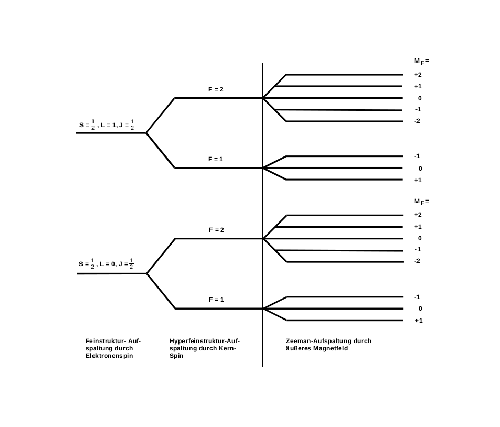
\includegraphics{optischesPumpen/img/aufspaltung.pdf}
  \caption{Hyperfeinstruktur- und Zeeman-Aufspaltung, beispielhaft für ein Alkali-Atom mit $I=\frac{3}{2}$.}
  \label{aufspaltung}
\end{figure}

\subsection{Optisches Pumpen}

Die Energieniveaus der inneren Schalen der Elektronenhülle sind vollstandig besetzt, die Besetzung der äußeren Schalen ist
temperaturabhängig. Im thermischen Gleichgewicht wird sie für zwei Niveaus mit den Energien $W_1$ und $W_2$ durch die
Boltzannsche Gleichung
\begin{align}
  \frac{N_2}{N_1} = \frac{g_2}{g_1}\frac{\exp(-W_2/kT)}{\exp(-W_1/kT)}
  \label{boltz}
\end{align}
beschrieben. $N_i$ sind die Besetzungszahlen der jeweiligen Zustände und die statistischen Gewichte $g_i$ sind ein Maß
dafür, wie viele Zustände es pro Energie $W_i$ gibt.

Der Begriff Optisches Pumpen bezeichnet eine Methode, mit der eine Abweichung von der in \autoref{boltz} gegebenen
Verteilung erzielt werden kann - zum Beispiel in Form einer Inversion, wo $N_2 > N_1$ ist.
Dafür wird Licht eingestrahlt, das gerade die nötige Energie besitzt, um ein Hüllenelektron vom Grundzustand in einen
angeregten Zustand zu versetzen. Für ein Alkali-Atom ist $J=\frac{1}{2}$, $M_\text{J}$ kann also nur $\pm \frac{1}{2}$
werden. Aufgrund der Auswahlregeln sind nur Übergänge mit $\Delta M = 0,\pm 1$ möglich.
Bei $\pi$-Übergangen mit $\Delta M = 0$ wird linear polarisiertes Licht emitiert und absorbiert, für $\sigma^\pm$-Übergänge
mit $\Delta M = \pm 1$ ist es rechtszirkular- bzw. linkszirkular-polarisiertes Licht.
Wird rechtszirkular-polarisiertes Licht in eine Zelle mit dem Dampf eines Alkali-Atom eingestrahlt, können aufgrund der
Beschränkung $\Delta M_\text{J}$ nur Elektronen aus dem energetisch niedrigeren Grundzustand angeregt werden, durch spontane
Emission aus dem angeregten Zustand, werden aber beide Grundzustände bevölkert. Das energieärmere Niveau wird fortlaufend
durch Einstrahlung von Licht geleert, das energetisch höhere, aus dem keine Elektronen angeregt werden können, wird gesättigt.
Als Resultat steigt der Transmissionskoeffizient asymptotisch gegen den Wert 1, da keine Elektronen mehr verfügbar sind, die
angeregt werden können.

\subsection{Messung der Zeeman-Aufspaltung}

Ein Elektron im angeregten Zustand kann durch spontane oder durch angeregte Emission in seinen Grundzustand zurückkehren.
Dabei ist letzteres bei Energien, die für Zeeman-Aufspaltung relevant sind, um 25 Größenordnungen wahrscheinlicher, da die
Übergangswahrscheinlichkeit für spontane Emission $\propto \nu^3$ ist.
Die Zeeman-Aufspaltung tritt nur bei angelgtem Magnetfeld auf, sodass auch nur bei externem Magnetfeld das optische Pumpen
durch Einstrahlen einer geeigneten Lichtquelle in stattfinden kann. Wird ein Magnetfeld angelegt, dass das Erdmagnetfeld gerade ausgleicht, findet keine Aufspaltung statt,
es tritt keine Inversion auf und der Transmissionskoeffizient sinkt.
Ein solcher Einbruch in der Intensität des Lichts tritt auch auf, wenn ein frequenzvariables Hochfrequenzfeld an die
Dampfzelle angelegt wird. Das Magnetfeld wird variiert und sobald es den Wert
\begin{equation}
  B_\text{m} = \frac{4\pi m_0}{\text{e}_0g_\text{J}}\nu
\end{equation}
erreicht, setzt induzierte Emission ein. Die Inversion wird aufgehoben, das eingestrahlte Licht kann wieder absorbiert werden
und der Transmissionskoeffizient fällt ab. Die geschieht jeweils für die beiden Rubidiumisotope bei unterschiedlichem
Magnetfeld.

\subsection{Quadratischer Zeeman-Effekt}

Wird die magnetische Flussdichte vergrößert, müssen bei der Berechnung der Übergangsenergie Terme höherer Ordnung von $B$
berücksichtigt werden, da nun die Spin-Bahn-Wechselwirkung relevant wird. Die Zeeman-Übergänge haben eine unterschiedliche
Energie und sind abhängig von $M_\text{F}$. Der Übergang von einem Zustand $M_\text{F}$ zu $M_\text{F}-1$ mit einer
Hyperfeinstrukturaufspaltung $\Delta E_\text{Hy}$ wird durch die Breit-Rabi-Formel beschrieben:
\begin{equation}
  U_\text{HF} = g_\text{F}\mu_\text{B}B + {g_\text{F}}^2{\mu_\text{B}}^2B^2\frac{1-2M_\text{F}}{\Delta E_\text{Hy}}
\end{equation}

\subsection{Transiente Effekte}

Wird das Hochfrequenzfeld schnell ein- und ausgeschaltet, präzediert der Kernspin um das effektive Magnetfeld. Die
Lamor-Frequenz $\\nu = \gamma B_\text{RF}$ mit dem gyromagnetischen Verhältnis $\gamma = g_\text{f}\frac{\mu_ß}{\text{h}}$
ist vom Lande-Faktor abhängig und somit für die beiden Rubidiumisotope verschieden. Das Verhältnis der Relaxationsperioden
$T = 1/\gamma B_\text{RF}$ ist dann
\begin{equation}
  \frac{T_{87}}{T_{85}} = \frac{\gamma_{85}}{\gamma_{87}}.
\end{equation}

\section{Versuchsaufbau und Durchführung}

\begin{figure}[h]
\centering
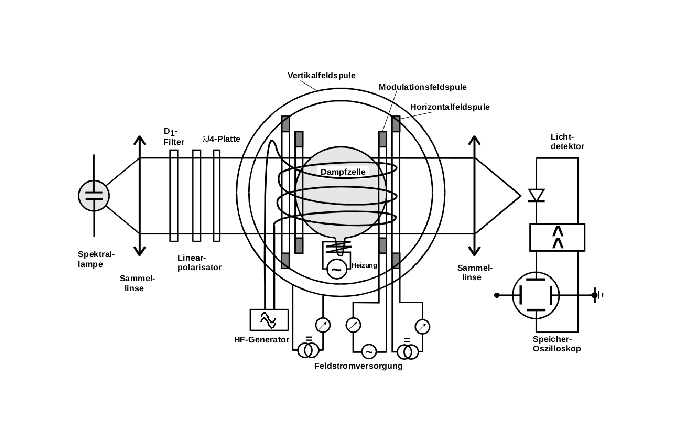
\includegraphics[scale=0.8]{/img/aufbau.pdf}
\caption{Schematischer Aufbau der Versuchsapparatur [1]}
\label{aufbau}
\end{figure}

Der Versuch wird mit dem Aufbau, der in \autoref{aufbau} schematisch dargestellt ist, durchgeführt. Dafür wird zunächst
Rubidium erhitzt, sodass sich die Dampfzelle damit füllt. Ein angelegtes Magnetfeld wird so lange variiert bis der Einbruch
in der Intensität des eingestrahlten Lichts möglichst schmal wird. Dadurch wird der Effekt des Erdmagnetfeldes kompensiert.
Zu diesem Zweck ist der gesamte Versuch parallel zum Erdmagnetfeld auszurichten. Das eingestrahlte Licht geht durch einen
Interferenzfilter, einen Polarisationsfilter und eine $\lambda/4$-Platte, um rechtszirkular-polarisiertes $D_1$-Licht zu
erhalten. Mit einer Sweep-Spule wird das Magnetfeld variiert, um die Stellen bestimmen zu können, wo induzierte Emission
einsetzt und der Transmissionskoffizient sinkt. Daraus wird die Stärke des Erdmagnetfeldes, die Lande-Faktoren und die
Kernspins der Rubidiumisotope berechnet. Aus der Amplitude der Pulse an den Resonanzstellen wird das Isotopenverhältnis
bestimmt. Durch Verändern der Amplitude des Hochfrequenzfeldes bei festgehaltener Frequenz wird das Verhältnis der
Relaxationsperioden bestimmt.

\section{Auswertung}
\subsection{Bestimmung der g-Faktoren und Horizontalkomponente der Erdmagnetfeld}
Zu Beginn wird die lokale horizontal Komponente des Erdmagnetfeldes und die Lande-Faktoren $g_F$ der Rb-Isotope, welche in der Dampfzelle enthalten sind, ermittelt.
Dafür werden die verschiedenen Frequenzen gegen die magnetischen Feldstärken in der jeweiligen Resonanz aufgetragen. Mittels einer linearen Ausgleichsrechnung werden die $g_F$ als Steigung und die horizontal Komponente als Ordinate identifiziert.

\begin{figure}[h]
\centering
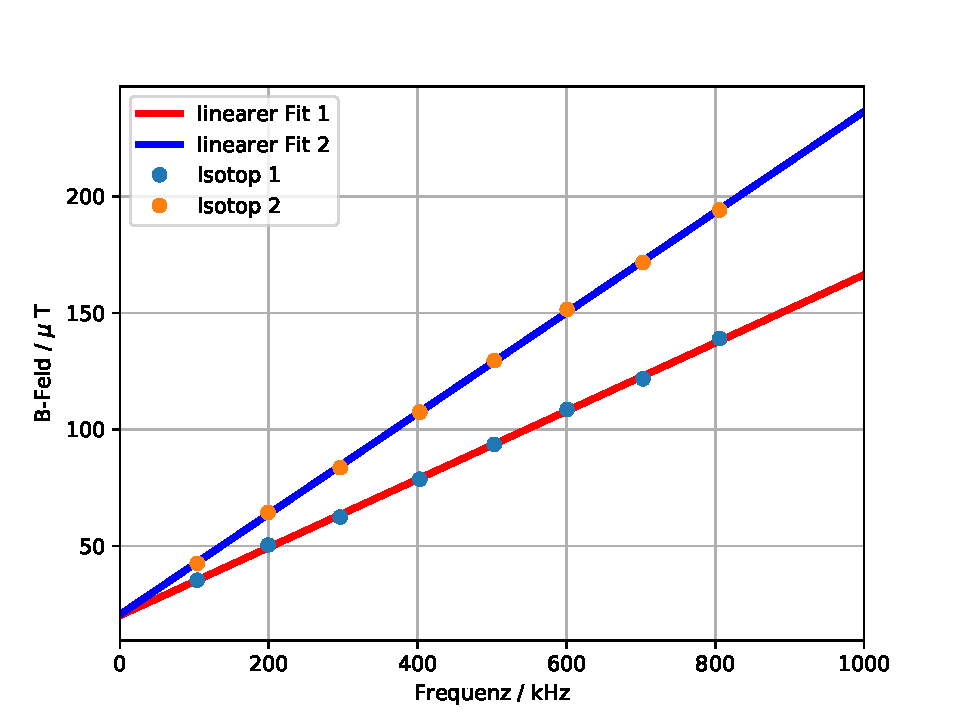
\includegraphics[scale=0.8]{img/plotLande.pdf}
\caption{Ausgleichsrechnung zur Bestimmung der Lande Faktoren der Rb-Isotope und der lokalen horizontal Komponente des Erdmagnetfeldes}
\label{aufbau}
\end{figure}

Mit dem Ansatz
\begin{equation}
f(x) = Ax + B
\end{equation}
folgt aus der Ausgleichsrechnung folgende Werte für die Koeffizienten A und B.

\begin{table}\centering\begin{tabular}{ccc} \toprule 
\centering
\caption{Ergebnisse für die Koeffizienten A und B der Ausgleichsrechnung.}
\label{tab:isoFit}
 & A / $\mu$T/kHz  & B / $\mu$T \\ \midrule
Isotop 1 & 0.146 $\pm$ 0.001 & 20.1 $\pm$ 0.7 \\
Isotop 2 & 0.216 $\pm$ 0.001 & 20.5 $\pm$ 0.6 \\
\bottomrule
\end{tabular}
\end{table}

Durch Koeffizientenvergleich mit gleichung 0.10 folgt für die Lande Faktoren

\begin{equation} 
g_{F1} = 0.488\pm0.005\,
label{eq:resG1}
\end{equation} 


und

\begin{equation} 
g_{F2} = 0.331\pm0.002\,
label{eq:resG2}
\end{equation} 


Außerdem lässt sich aus der Ordinate die horizontalkomponente des Erdmagnetfeldes bestimmen,
welche sich zu

\begin{equation} 
B_\text{h} = 20.3\pm0.5\,\mu\text{T}
\end{equation} 


errechnet.

\subsection{Bestimmung der Kernspins}
Zur bestimmung des Kernspins muss Gleichung 2.8 für die zwei berechneten g-Faktoren gelöst werden. Dafür werden beide Seiten der Gleichung in Abhängigkeit
des Kernspins I aufgetragen. Der Punkt an den sich beide Kurven schneiden, zeigt den Kernspin des zu Untersuchenden Isotope an.

\begin{figure}[h]
\centering
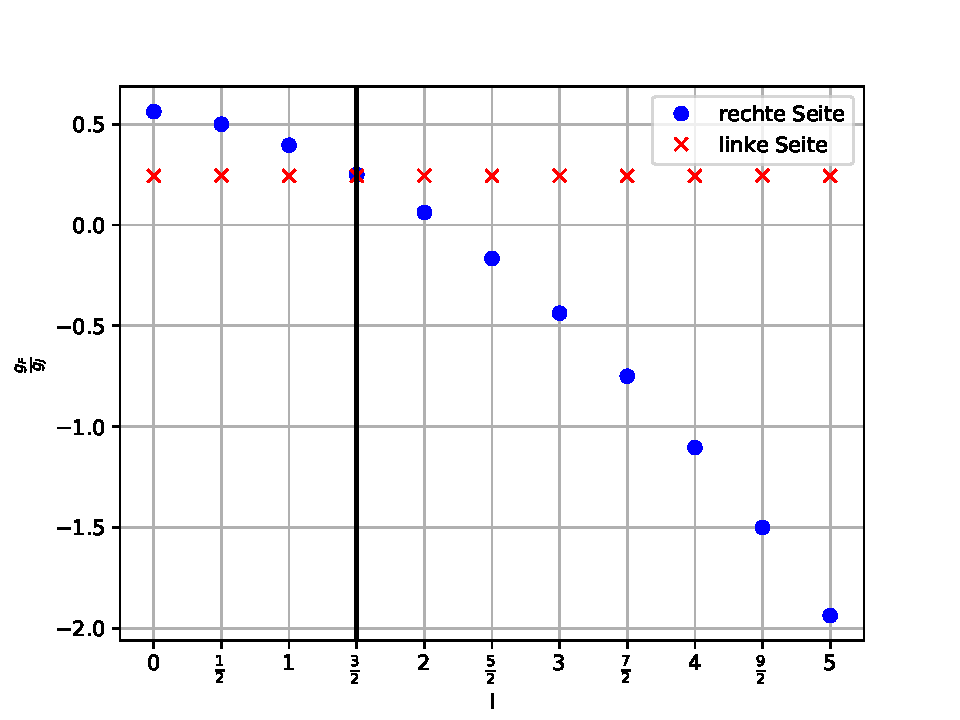
\includegraphics[scale=0.8]{img/coreSpin1.pdf}
\caption{grafische Lösung zur berechnung des Kernspins von Isoptop 1}
\label{LandeIso1}
\end{figure}

\begin{figure}[h]
\centering
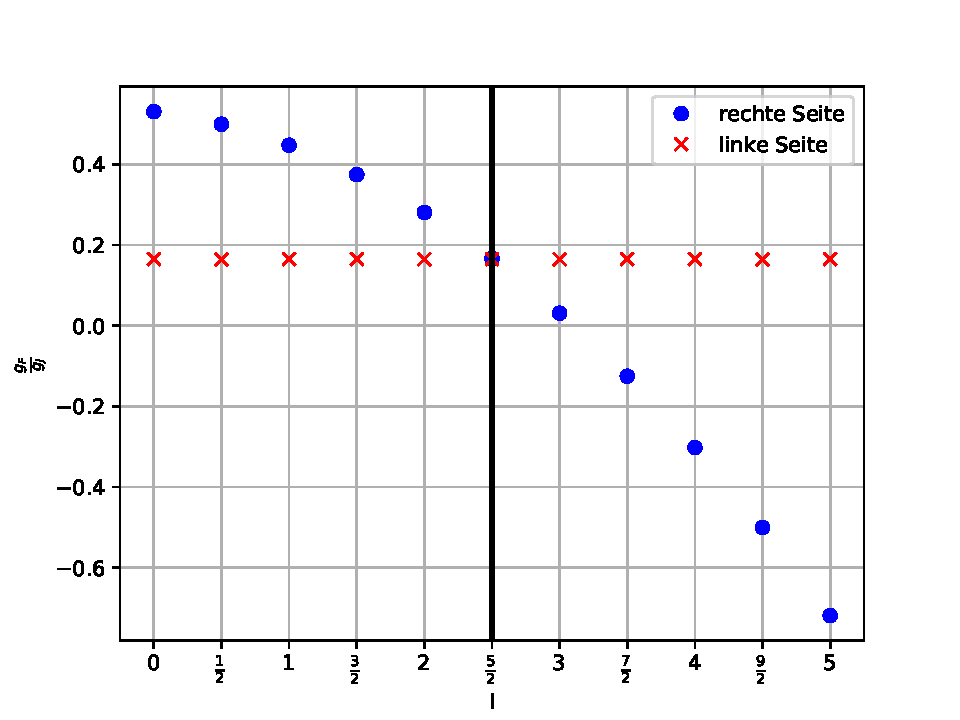
\includegraphics[scale=0.8]{img/coreSpin2.pdf}
\caption{grafische Lösung zur berechnung des Kernspins von Isoptop 2}
\label{LandeIso2}
\end{figure}

Aus den errechneten g-Faktoren und Kernspins können wir Isotop 1 als Rb87 und Isotop 2 als Rb85 identifizieren.


\subsection{Bestimmung des Isotopenverhältnisses}
In Abbildung \autoref{resonanz} ist das Signalbild dargestellt, welches die Resonanzen zu festen
Feldstärken zeigt.

\begin{figure}[h]
\centering
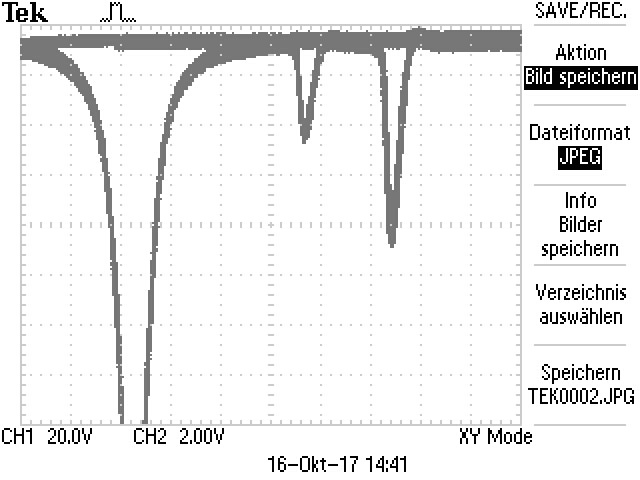
\includegraphics[scale=0.8]{img/TEK0002.JPG}
\caption{Abbildung der Resonanzen}
\label{resonanz}
\end{figure}


Aus dem Amplitudenverhältnis der Resonanzen wird das Isotopenverhältnis in der
Dampfzelle ermittelt. Dafür wird die Tiefe der Resonanzen in Pixel bestimmt.
Eine Messung der Tiefe der Resonanzen mit gimp liefert für die erste Resonanz (von links)

\begin{equation} 
h_1 = 108.0\pm1.1\,\text{px}
\end{equation} 


für die zweite Resonanz

\begin{equation} 
h_2 = 213.0\pm2.1\,\text{px}
\end{equation} 


und für das Amplitudenverhältnis

\begin{equation} 
r = 0.507\pm0.007\,
\end{equation} 


Bei der Kalkulation des Amplitudenverhältnisses wurde ein Ablesefehler von 1 Prozentpunkt
angesetzt.

\subsection{Abschätzung des quadratischen Zeemann-Effektes}
Für starke Magnetfelder verhält sich die Übergangsenergie $U_{HF}$ nicht mehr proportional zu B, um diese Abweichung zu berücksichtigen, ist es notwenig Terme höherer Ordnung zu betrachten.
Im folgenden wird die größe des quadratischen Termes für die genutzen Feldstärken abgeschätzt. Wird der quadratische Term explizit ausgewertet zeigt sich, dass der quadratische Zeeman-Effekt
in diesem Fall proportional zu $10^{-33}$ ist.

\subsection{transiente Effekte}
Im folgenden werden die transienten Effekte betrachtet. Ein typisches Signalbild ist Abbildung \ref{sigPic} zu entnehmen.

\begin{figure}[h]
\centering
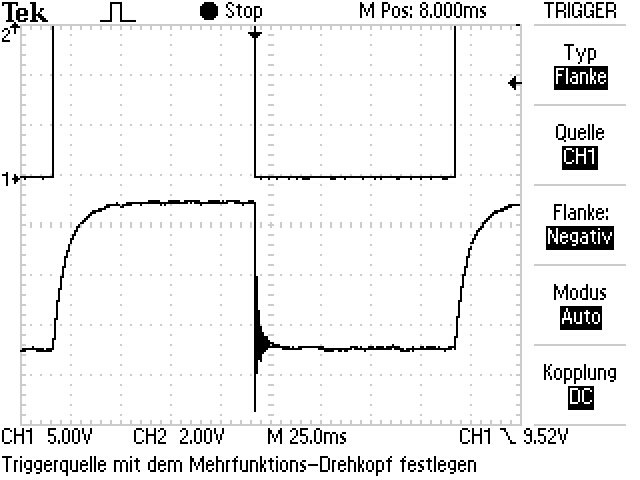
\includegraphics[scale=0.8]{img/TEK0019.JPG}
\caption{Signalbild}
\label{sigPic}
\end{figure}

Es wird die RF-Amplitude gegen die Periode aufgetragen und anschließend eine Ausgleichsrechnung mit Hilfe der Funktion

\begin{equation}
f(x) = A + \frac{B}{(C-1)^{-1}}
\end{equation}

durchgeführt.

Es ergeben sich die Abbildungen \ref{trans1} und \ref{trans2}

\begin{figure}[h]
\centering
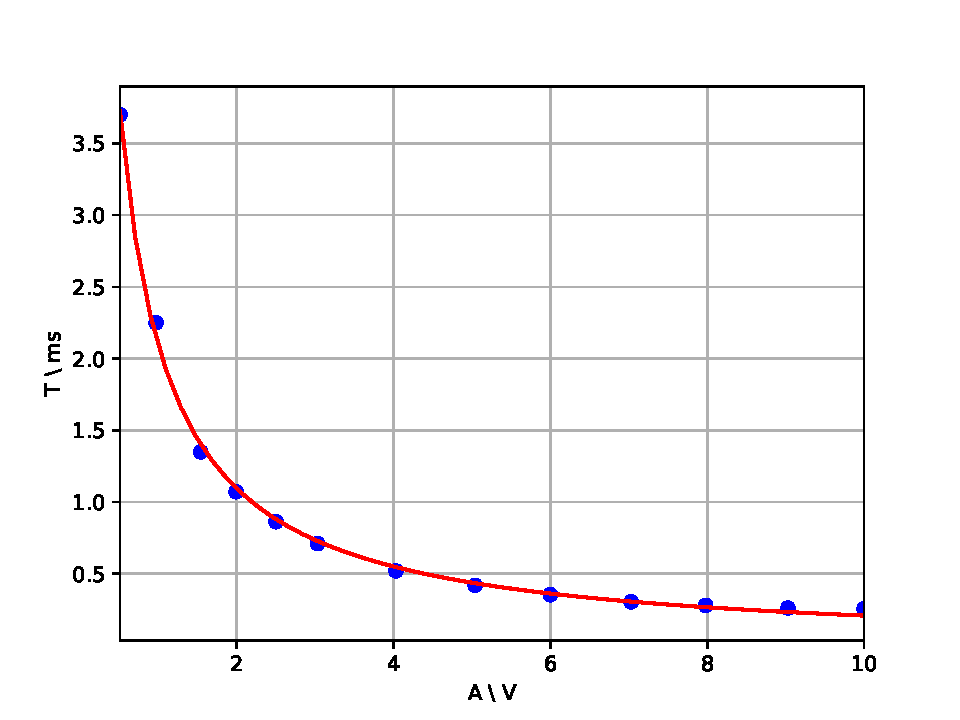
\includegraphics[scale=0.8]{img/trans1.pdf}
\caption{Ausgleichsrechnung Isotop 1}
\label{trans1}
\end{figure}

\begin{figure}[h]
\centering
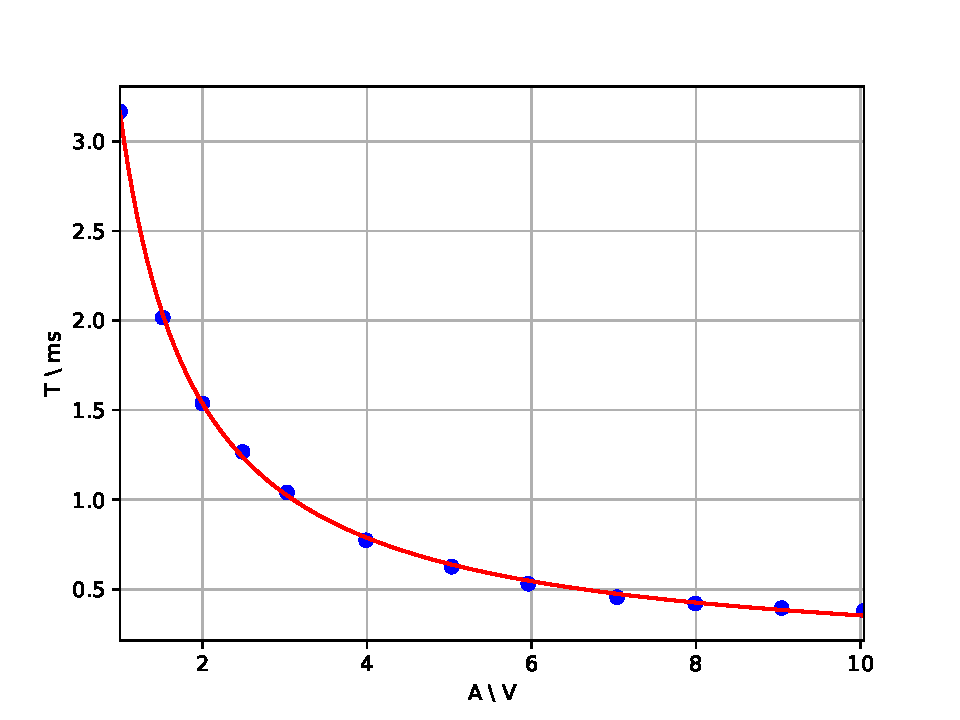
\includegraphics[scale=0.8]{img/trans2.pdf}
\caption{Ausgleichsrechnung Isotop 2}
\label{trans2}
\end{figure}

Die Ausgleichsrechnung liefert für \ref{trans1}
\begin{table}[h!]
\centering
\begin{tabular}{cc} \toprule
\centering
A & -0,03 $\pm$ 0,03 \\
B & 2,4 $\pm$ 0,1 \\
C & -0,13 $\pm$ 0,03 \\
\bottomrule
\end{tabular}
\end{table}

und für \ref{trans2}

\begin{table}[h!]
\centering
\begin{tabular}{cc} \toprule
\centering
A & 0,07 $\pm$ 0,01 \\
B & 2,79 $\pm$ 0,07 \\
C & 0,09 $\pm$ 0,02 \\
\bottomrule
\end{tabular}
\end{table}

Der Quotient der Fitparameter B der beiden Ausgleichsrechnungen liefert

\begin{equation}
\frac{b_{2}}{b_{1}} = 1,17 \pm 0,06
\end{equation}

\section{Diskussion}
Die errechneten g-Faktoren für Rb85 und Rb87 mit $g_{F,85} = 0,488 $\pm$ 0,005$ und
$g_{F,87} = 0,331 $\pm$ 0,002$ stimmen mit guter Genauigkeit mit den Theoriewerten von $\frac{1}{2}$ und $\frac{1}{3}$ überein.
Auch der Wert für die horizontal Komponente des Erdmagnetfeldes scheint unter Berücksichtigung der Größenordnung plausiebel zu sein.

Der Vergleich der Kernspins mit den Literaturwerten liefert ebenso eine zufriedenstellende Übereinstimmung.
Für Rb85 finden wir einen Kernspin von  I_{Rb,85} = $\frac{5}{2}$ und für Rb87 einen Kernspin von I_{Rb,87} = $\frac{3}{2}$, was im wesentlichen den Literaturwerten \cite{coreSpin} entspricht.

Das errechnete Isotopenverhältnis von r = 0,507 weicht signifikant vom Literaturwert von r = 0,386 \cit{isoVer} ab. Als mögliche Fehlerquelle
sei hier eine möglicherweise nicht komplett abgedunkelte Apparatur genannt. In diesem Fall hätte das einfallende Restlicht
einen Offset in der Amplitudentiefe der Resonanzen bewirkt.

Auch könnte die Speicherung als JPEG und die weitere Verarbeitung mit gimp einen Fehler begründen.

Die Abschätzung des quadratischen Zeemann-Effektes zeigt, das der quadratische Term bei den verwendeten Feldstärken drei Größenordnungen kleiner ist als der lineare Term. Daher kann der Einfluss des quadratischen Terms in guter Näherung vernachlässigt werden.

Der Theoriewerte des Verhältnisses $\frac{b_{87}}{b_{85}}$ ist 1,5 \cite{FP}. Somit weicht das Messergebnis von $\frac{b_{87}}{b_{85}} = 1,17 \pm 0,06$ um 22 Prozenpunkte vom Theoriewert ab.
Dieser Abweichung lässt sich damit begründen, dass das Zählen der Perioden nicht mit absoluter Genauigkeit möglich war.

\printbibliography


\backmatter
\printbibliography

\end{document}
